% Session 9 -- three regimes of translational symmetry, three kinds of eigenstate,
% Placement: sec. "Disorder and Anderson localization", after equation (9.12).
% Rendered by figures/blender/s09f06_localization.py, labels in figures/overlays/s09f06_localization.tex.
\begin{aqmfigure}{fig:s09:localization}{The three regimes of Section 9.10, shown through their
effect on an eigenstate of a chain of $N=89$ sites, with the weight $|\psi_i|^2$ of each site as a
column. (a) With a periodic potential every eigenstate is a Bloch wave, with weight exactly $1/N$ on
every site, and this height becomes smaller as the chain grows. (b) At the self-dual point of the
quasiperiodic model the state is neither extended nor localized. It has structure on every length
scale at the same time, with large peaks and smaller copies of the same pattern between them, and
this state is called critical, or multifractal. (c) With really random disorder the state is
concentrated on a few sites and it is strictly zero, to numerical precision, over most of the chain.
\emph{Note the three different vertical scales.} For this reason we need a number and not a visual
check, and this number is the inverse participation ratio (9.12). (d) The IPR separates the three
regimes clearly by how it scales with system size, with $\mathrm{IPR}\sim1/N$ for extended states,
$\mathrm{IPR}\sim O(1)$ for localized ones, and an anomalous power $N^{-\tau}$ with $0<\tau<1$ for
the critical state between them, here computed for $N=34$ to $610$. On a log-log plot these are
three straight lines with three different slopes.}
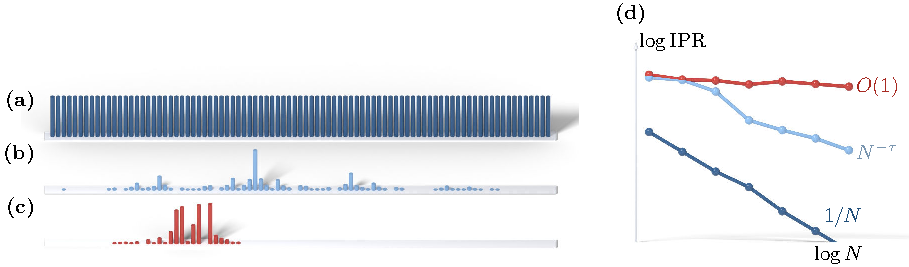
\includegraphics{figures/pdf/s09f06_localization.pdf}
\end{aqmfigure}
